\documentclass[11pt,a4paper]{ctexart}

\usepackage[a4paper,margin=2.15cm,headheight=15pt]{geometry}
\usepackage{fontspec}
\usepackage{xeCJK}
\usepackage{graphicx}
\usepackage{xcolor}
\usepackage{booktabs}
\usepackage{longtable}
\usepackage{tabularx}
\usepackage{array}
\usepackage{multirow}
\usepackage{enumitem}
\usepackage{hyperref}
\usepackage{fancyhdr}
\usepackage{titlesec}
\usepackage[most]{tcolorbox}
\usepackage{pdflscape}
\usepackage{caption}
\usepackage{microtype}
\usepackage{amsmath}
\usepackage{amssymb}
\usepackage{pifont}

\setCJKmainfont{Noto Serif CJK SC}
\setCJKsansfont{Noto Sans CJK SC}
\setmainfont{Noto Serif CJK SC}
\setsansfont{Noto Sans CJK SC}
\setmonofont{DejaVu Sans Mono}

\definecolor{navy}{HTML}{102A43}
\definecolor{blue}{HTML}{2563EB}
\definecolor{bluebg}{HTML}{EFF6FF}
\definecolor{green}{HTML}{0F766E}
\definecolor{greenbg}{HTML}{ECFDF5}
\definecolor{amber}{HTML}{B45309}
\definecolor{amberbg}{HTML}{FFFBEB}
\definecolor{red}{HTML}{B91C1C}
\definecolor{redbg}{HTML}{FEF2F2}
\definecolor{slate}{HTML}{486581}
\definecolor{line}{HTML}{CBD5E1}
\definecolor{light}{HTML}{F8FAFC}

\hypersetup{
  colorlinks=true,
  linkcolor=navy,
  urlcolor=blue,
  citecolor=blue,
  pdftitle={Agent Skill Acquisition Security: Related Work Review},
  pdfsubject={导师版文献综述},
  pdfauthor={Skill Acquisition Barrier Research}
}

\pagestyle{fancy}
\fancyhf{}
\fancyhead[L]{\small\sffamily Agent Skill Acquisition Security}
\fancyhead[R]{\small\sffamily Related Work Review · 2026-07-20}
\fancyfoot[C]{\small\thepage}
\renewcommand{\headrulewidth}{0.4pt}
\renewcommand{\footrulewidth}{0pt}

\titleformat{\section}{\Large\bfseries\sffamily\color{navy}}{\thesection}{0.8em}{}
\titleformat{\subsection}{\large\bfseries\sffamily\color{navy}}{\thesubsection}{0.7em}{}
\titleformat{\subsubsection}{\normalsize\bfseries\sffamily\color{green}}{\thesubsubsection}{0.6em}{}
\titlespacing*{\section}{0pt}{1.2em}{0.65em}
\titlespacing*{\subsection}{0pt}{1.0em}{0.45em}

\setlength{\parindent}{2em}
\setlength{\parskip}{0.28em}
\setlist[itemize]{leftmargin=1.7em,itemsep=0.2em,topsep=0.3em}
\setlist[enumerate]{leftmargin=1.8em,itemsep=0.25em,topsep=0.3em}
\renewcommand{\arraystretch}{1.28}
\captionsetup{font=small,labelfont=bf}

\newcommand{\yes}{\textcolor{green}{\ding{51}}}
\newcommand{\no}{\textcolor{red}{\ding{55}}}
\newcommand{\partialc}{\textcolor{amber}{\ding{108}}}
\newcommand{\arxiv}[1]{\href{https://arxiv.org/abs/#1}{arXiv:#1}}
\newcommand{\code}[1]{\texttt{#1}}
\newcolumntype{Y}{>{\raggedright\arraybackslash}X}
\newcolumntype{L}[1]{>{\raggedright\arraybackslash}p{#1}}
\newcolumntype{C}[1]{>{\centering\arraybackslash}p{#1}}

\newtcolorbox{executivebox}{
  enhanced, breakable, colback=greenbg, colframe=green,
  boxrule=0.9pt, arc=2mm, left=3mm, right=3mm, top=2mm, bottom=2mm
}
\newtcolorbox{warningbox}{
  enhanced, breakable, colback=amberbg, colframe=amber,
  boxrule=0.8pt, arc=2mm, left=3mm, right=3mm, top=2mm, bottom=2mm
}
\newtcolorbox{papercard}[2][]{
  enhanced, breakable, colback=white, colframe=blue,
  colbacktitle=bluebg, coltitle=navy, fonttitle=\bfseries\sffamily,
  title={#2}, boxrule=0.7pt, arc=2mm,
  left=3mm, right=3mm, top=2mm, bottom=2mm,
  before skip=6pt, after skip=7pt, #1
}
\newtcolorbox{relationbox}[1]{
  enhanced, breakable, colback=light, colframe=line,
  title={#1}, coltitle=navy, fonttitle=\bfseries\sffamily,
  boxrule=0.6pt, arc=1.5mm, left=3mm, right=3mm, top=2mm, bottom=2mm
}

\begin{document}

\begin{titlepage}
  \pagecolor{light}
  \vspace*{2.2cm}
  {\sffamily\bfseries\fontsize{25}{33}\selectfont\color{navy}
  \mbox{Agent Skill Acquisition Security}\\[0.25cm]
  Related Work 详细综述\par}
  \vspace{0.8cm}
  {\Large\sffamily\color{slate}
  从能力缺口、发现、安装到调用与载荷\par}
  \vspace{1.5cm}

  \begin{tcolorbox}[colback=white,colframe=green,boxrule=1.1pt,arc=3mm,left=5mm,right=5mm,top=4mm,bottom=4mm]
  \large
  \textbf{综述结论：}现有研究已覆盖显式安装请求下的真实安装/调用，也已覆盖恶意搜索证据诱导出的安装命令。尚未被系统量化的是：\textbf{用户只给普通任务时，agent 是否因能力缺口自主发起检索并实际完成第三方 skill 安装，以及该过程如何沿完整攻击链逐段衰减。}
  \end{tcolorbox}

  \vfill
  \begin{tabular}{@{}ll@{}}
  \textbf{文献截止日期：} & 2026 年 7 月 20 日 \\
  \textbf{核心时间范围：} & 近一年；方法祖先回溯至 2024 年 \\
  \textbf{核对原文：} & 44 篇论文 / 技术报告 \\
  \textbf{研究项目：} & Skill Acquisition Barrier \\
  \textbf{文档用途：} & 导师独立阅读、研究定位与实验设计讨论
  \end{tabular}
  \vspace{0.8cm}
\end{titlepage}
\nopagecolor

\pagenumbering{roman}
\tableofcontents
\clearpage
\pagenumbering{arabic}

\section{执行摘要}

\subsection{研究对象}

Agent Skills 是一种可分发的能力包：通常包含自然语言指令文件（如 \code{SKILL.md}）、可执行脚本、参考资料和资源。与一次性的 prompt 或单个 API tool 不同，skill 会被发现、安装、加载并在后续任务中复用，因此同时具有\textbf{自然语言控制面、软件供应链和持久权限}三类风险。

本研究关心的不是单纯“恶意 skill 装进去后会不会作恶”，而是更完整的问题：

\begin{executivebox}
在具备搜索和安装能力的 LLM agent 中，恶意 skill 从公开市场进入可用能力集合、随后被调用并产生危害的真实瓶颈在哪里？用户未明确要求安装时，agent 是否会因为普通任务中的能力缺口而自主完成 acquisition？
\end{executivebox}

\subsection{文献形成的三块证据}

\begin{enumerate}
  \item \textbf{Post-load 执行已充分。} Skill-Inject、Poise、SkillTrojan、BadSkill 等表明，一旦 skill 已加载或已被信任，恶意规程、脚本和后门可获得高攻击成功率；此处不宜再作为主要 novelty。
  \item \textbf{库内发现与同类选择已充分。} IPI、ToolHijacker、ToolTweak、Semantic Supply-chain、MPMA 表明，检索排序、name/description、候选偏好均可被显著操纵；但这些工作通常条件化在恶意条目已进入 corpus、registry 或 tool library。
  \item \textbf{安装环已被部分而非完整覆盖。} HalluSquatting 已在用户明确要求 \code{install X} 时完成真实 marketplace 安装与调用；SearchGEO 已量化安装命令输出；Skills That Don't Exist 已展示幻觉推荐后的单例安装；SCR 已显示信任背书能大幅提高下游有害安装。它们共同推翻“从未有人测 install”的宽泛表述，但仍没有形成普通任务触发的自主 acquisition 全链 benchmark。
\end{enumerate}

\subsection{当前最稳的研究定位}

\begin{executivebox}
\textbf{Task-induced Autonomous Skill Acquisition：}用户只提出正常任务、不说“安装某 skill”；agent 自己识别能力缺口，搜索第三方能力，发出并实际执行安装，随后调用该能力。评测把模型意图、编排器解析、实际安装、调用、载荷和任务效用拆开报告。
\end{executivebox}

因此，本项目不应声称：第一次研究 skill 安装、第一次做 skill marketplace E2E、或第一次测 install ASR。可防守的贡献是：\textbf{S0 自主触发条件 + executed install + 完整分段条件概率 + 模型/编排器归因。}

\subsection{主张—证据总表}

\begin{center}
\small
\begin{tabularx}{\textwidth}{L{4.0cm}Y L{4.0cm}}
\toprule
\textbf{可写入论文的主张} & \textbf{主要证据} & \textbf{必须保留的边界} \\
\midrule
恶意内容首先要进入候选/上下文 & IPI；ToolHijacker；Semantic Supply-chain & 这些结果不直接等于安装成功 \\
已加载 skill 的 post-load 风险很高 & Skill-Inject；Poise；SkillTrojan；BadSkill & 不能与 pre-load 成功率横比 \\
显式安装请求可以被真实劫持 & HalluSquatting & 用户已经明确授权安装 \\
伪证据可诱导安装命令 & SearchGEO & 命令输出不等于执行 \\
推荐幻觉可形成 name-squatting 面 & Skills That Don't Exist & 大规模实验主要测 recommendation \\
信任转移能提高有害安装 & SCR-TrustLift & 下游安装请求仍被显式呈现 \\
普通任务触发的自主实装仍缺系统基准 & 本综述对 44 篇原文的阶段核对 & 应写“尚缺系统量化”，不写绝对无人研究 \\
\bottomrule
\end{tabularx}
\captionof{table}{研究主张、证据及边界。}
\end{center}

\clearpage
\section{综述范围与阅读方法}

\subsection{时间范围与文献池}

本报告以 2025 年 7 月至 2026 年 7 月的近一年工作为核心，并向前回溯至 2024 年，以纳入 tool-integrated agent 间接注入的基准祖先。截止 2026 年 7 月 20 日，共核对 44 篇原始 PDF。由于 Agent Skills 规范在 2025 年末才快速成形，绝大多数直接工作集中在 2026 年。

检索与纳入围绕以下关键词和引用链展开：\emph{agent skills, skill marketplace, skill install, autonomous acquisition, SKILL.md, tool selection, MCP poisoning, indirect prompt injection, skill supply chain, registry discovery, malicious skills, skill scanner}。此外沿直接竞品的 related-work 与参考文献回溯方法祖先。

本报告属于\textbf{结构化叙述综述}，不是注册协议下的系统综述或 meta-analysis。原因是领域更新极快、术语尚未统一、许多工作仍为预印本，且 ASR 的分母、初始条件和成功终点差异极大，无法直接汇总成一个加权平均。

\subsection{纳入标准}

\begin{itemize}
  \item 直接研究 Agent Skills / SKILL.md / skill marketplace 的架构、安全、测量、攻击或防御；
  \item 研究 tool/MCP 的检索、选择、偏好操纵或间接注入，且机制可迁移到 S0--S3；
  \item 研究文档权威、信任转移、依赖组合或安装决策，能解释 Stage2 通道；
  \item 少量研究 autonomous skill generation/mining，仅用于澄清“acquisition”术语歧义。
\end{itemize}

\subsection{关系标签}

\begin{tabularx}{\textwidth}{C{1.4cm}L{3.4cm}Y}
\toprule
\textbf{标签} & \textbf{类别} & \textbf{判定方式} \\
\midrule
D & 直接竞品 & 覆盖真实 install、安装命令、skill 推荐交付或与主 threat model 高度重合 \\
C & 阶段证据 & 直接支持 S0/S1/S2/S3 某一段的可攻击性或指标设计 \\
E & 生态证据 & 证明市场规模、恶意 skill 在野存在、分发或依赖风险 \\
M & 方法祖先 & 提供 barrier、IPI、tool-agent benchmark 等研究结构 \\
F & 防御/治理 & 研究扫描、运行时审计、权限或生命周期治理 \\
A & 邻接工作 & 术语相近或提供工程背景，但不直接回答安装决策 \\
\bottomrule
\end{tabularx}

\subsection{为什么不能直接比较 ASR}

不同论文中的“成功”可能分别是：毒文档进入 top-$k$、恶意工具被选中、模型输出安装命令、skill 实际写入本地、恶意 skill 被调用、载荷生效、或载荷生效且用户任务仍完成。除此之外，初始状态还可能是“已加载”“已在库”“已在 registry”“用户明确说安装”“用户只问普通任务”。本报告因此始终同时记录：

\begin{equation*}
\text{Initial State} + \text{Trigger} + \text{Action Executed} + \text{Evaluation Endpoint}.
\end{equation*}

\begin{warningbox}
同名 ASR 不代表同一随机变量。例如 Skill-Inject 的 ASR 条件化在 skill 已加载；SearchGEO 的 install ASR 终止于文本命令输出；HalluSquatting 的 E2E 条件化在显式安装请求。它们都不能与普通任务触发的自主 acquisition 成功率直接横比。
\end{warningbox}

\section{生命周期与概念边界}

\subsection{Skill、Tool 与 MCP}

\begin{tabularx}{\textwidth}{L{2.5cm}Y Y Y}
\toprule
 & \textbf{Agent Skill} & \textbf{Tool / Function} & \textbf{MCP Server} \\
\midrule
基本形态 & 指令、代码、资料组成的文件目录 & 带 schema 的可调用函数 & 暴露资源与工具的协议服务 \\
加载方式 & metadata 常驻，正文/资源按需加载 & schema 通常直接进入候选 & client 连接后获得 server tools \\
主要信任面 & 自然语言规程 + 本地脚本 + 持久复用 & name/description + 参数与返回 & server 描述、调用、返回、跨服务组合 \\
与本研究关系 & 主对象：发现、安装、加载、调用 & selection 与返回注入的方法对照 & 偏好操纵、false-error、tool transfer 的机制菜单 \\
\bottomrule
\end{tabularx}

Skills Survey（\arxiv{2602.12430}）用 progressive disclosure 描述三层加载：metadata 常驻、指令按相关性加载、scripts/assets 按需使用。这解释了为什么供应链风险不仅发生在 payload：metadata 决定“是否相关”，正文决定“遵循什么规程”，资源决定“执行什么代码”。

\subsection{S0--S3 操作化}

\begin{table}[htbp]
\small
\begin{tabularx}{\textwidth}{C{1.2cm}L{3.1cm}Y L{4.1cm}}
\toprule
\textbf{阶段} & \textbf{核心问题} & \textbf{建议指标} & \textbf{主要文献覆盖} \\
\midrule
S0 & agent 是否因能力不足产生扩展意图？ & \code{gap\_triggered}；search intent & 架构/自改进工作有概念，安全实证最薄弱 \\
S1 & 恶意 skill 是否进入 top-$k$/候选？ & \code{retrieved@k}, rank, pairwise win & IPI、ToolHijacker、Semantic SC \\
S2 & agent 是否采纳并真正安装？ & recommended、emitted、parsed、executed、on-disk & HalluSquatting、SearchGEO、SCR、Skills Don't Exist 部分覆盖 \\
S3 & 安装后是否调用、危害且任务仍成功？ & invoked、payload、task\_ok & Skill-Inject、Poise、ToolTweak、后门类 \\
\bottomrule
\end{tabularx}
\caption{本研究的生命周期分解。}
\end{table}

\begin{landscape}
\thispagestyle{empty}
\begin{figure}[p]
\centering
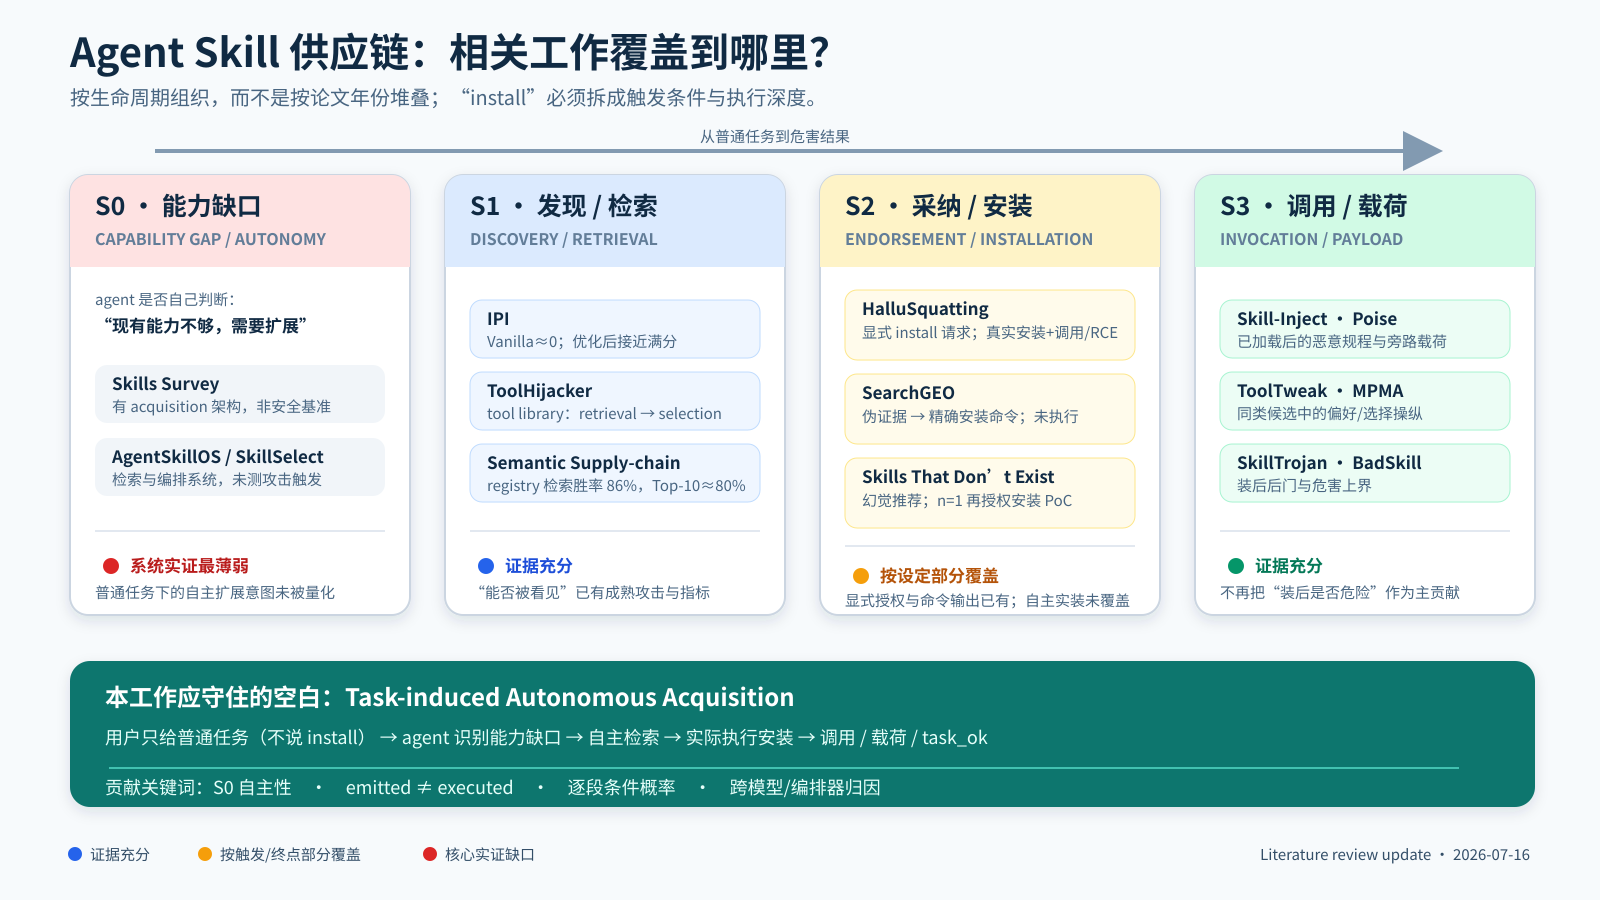
\includegraphics[width=0.98\linewidth]{figures/related_work_lifecycle_map.png}
\caption{Agent Skill 供应链相关工作覆盖图。蓝色表示已有充分攻击与指标；黄色表示安装环按触发方式和评测终点部分覆盖；红色表示普通任务下的自主扩展意图仍缺系统实证。}
\end{figure}
\end{landscape}

\clearpage
\section{领域演进：2024--2026}

\begin{longtable}{L{1.5cm}L{4.0cm}L{5.3cm}L{4.2cm}}
\toprule
\textbf{时期} & \textbf{代表工作} & \textbf{领域推进} & \textbf{对本研究的意义} \\
\midrule
\endfirsthead
\toprule
\textbf{时期} & \textbf{代表工作} & \textbf{领域推进} & \textbf{对本研究的意义} \\
\midrule
\endhead
2024 & InjecAgent；AgentDojo & 建立 tool-integrated agent 的 IPI benchmark，区分用户任务效用与攻击目标 & 工具返回可成为权威通道；task utility 必须进入成功定义 \\
2025 上半年 & ToolHijacker；MPMA & 从“恶意返回”推进到 tool retrieval/selection 与 MCP preference manipulation & S1 与候选内选择可被优化，但默认工具已在库/服务已可见 \\
2025 下半年 & MCPTox；ToolTweak；MSB；早期 Skill PI & 工具描述投毒、同类选择、MCP 多阶段 taxonomy；Agent Skills 供应链开始独立成面 & 建立 Stage2/3 方法菜单；false-error、广告偏好和 metadata 攻击有先例 \\
2026 一季度 & Skills Survey；Do Not Mention；Skill-Inject；AgentSkillOS；Repository Context & Skill 生态迅速规模化；出现大规模在野测量与装后攻击 benchmark & 证明风险现实，但多数工作仍从已存在/已加载开始 \\
2026 二季度 & Semantic SC；Poise；SCR；动态恶意 skill、PhantomSkill、ShareLock；扫描器 & lifecycle、组合信任、旁路载荷、运行时变毒和防御成为主线 & S1/S3 更强；S2 获得信任转移证据；安装不应再写成整体空白 \\
2026 七月 & HalluSquatting；SearchGEO；Skills Don't Exist；Cloak and Detonate & 真实安装 E2E、命令背书、幻觉推荐交付和 scanner evasion 直接出现 & 迫使 novelty 收窄为 task-induced autonomous acquisition 与逐段执行归因 \\
\bottomrule
\end{longtable}

\section{核心文献深读：Barrier、发现与选择}

\begin{papercard}{IPI：Overcoming the Retrieval Barrier（\arxiv{2601.07072}，2026）}
\textbf{研究问题。} 既有间接提示注入常把恶意文档直接放进上下文；真实检索系统中，恶意内容是否首先能进入 top-$k$？

\textbf{设定与方法。} 攻击者把含恶意指令的文本放入大规模 corpus，用 Cross-Entropy Method（CEM）黑盒优化一小段 trigger，使 embedding retriever 更可能召回它；覆盖 11 个数据集与多种 embedding 模型。

\textbf{指标与结果。} Vanilla 在所有数据集上检索失败；CEM 的平均 Recall@5 约 95.6\%，多数据集达到近 100\%。论文进一步把检索成功接到多 agent 危害，报告最高约 80\% 的工作流攻击成功。

\textbf{它证明什么。} 攻击链中被前人默认通过的中间门，可能才是真实瓶颈；检索门也可被系统优化打穿。

\textbf{与本研究关系。} 这是 Acquisition Barrier 的叙事祖先和 S1 方法先例。它不测 skill 安装，也不证明 S2 难易。
\end{papercard}

\begin{papercard}{ToolHijacker：Prompt Injection Attack to Tool Selection（\arxiv{2504.19793}，2025）}
\textbf{研究问题。} 大型 tool library 常先检索再由 LLM 选择；攻击者能否在 no-box 条件下注入恶意 tool document，操纵两段流程？

\textbf{设定与方法。} 恶意 tool document 已在 library 中；作者分别优化 retrieval objective 与 selection objective，并使用 shadow pipeline 构造可迁移文本。评测覆盖 8 个 LLM 和 4 个 retriever。

\textbf{关键结果。} 在 MetaTool 等设定中，攻击命中率可达到 100\%；自动优化显著优于手工注入。StruQ、SecAlign、已知答案检测、perplexity 等防御均不足以稳定阻断。

\textbf{它证明什么。} tool selection 不是单一步骤；只有候选内 persuasion 而没有 retrieval，不能构成完整库内劫持。

\textbf{与本研究关系。} 强支持 S1 + S3a 分解，但初始条件是恶意文档已进入 tool library，不覆盖从市场到本地的 install。
\end{papercard}

\begin{papercard}{Semantic Supply-chain on SKILL.md Registry（\arxiv{2605.11418}，2026）}
\textbf{研究问题。} \code{SKILL.md} 是否只是文档，还是会操作性地影响 registry 的发现、选择与治理？

\textbf{设定与方法。} 使用真实 ClawHub skills 和现实 registry 机制，分为 Discovery、Selection、Governance 三段；仅修改 \code{SKILL.md} 语义文本，不改变可执行代码。

\textbf{关键结果。} Discovery 触发器达到 86.14\% pairwise win 和 80\% Top-10 placement；只改 description 的功能等价对抗版本，在四模型 paired trials 中平均被选中 77.6\%；治理规避使恶意 skill 在 36.5\%--100\% 情况下逃过 blocking verdict。

\textbf{它证明什么。} registry lifecycle 本身是安全边界；上架、排序、曝光和选择均可被自然语言操纵。

\textbf{与本研究关系。} 是最强 pre-load 阶段证据，但终点仍是 registry ranking / candidate selection / governance，不单独报告 agent 实际执行 install。
\end{papercard}

\begin{papercard}[fontupper=\small]{ToolTweak 与 MPMA：候选内偏好操纵（\arxiv{2510.02554}；\arxiv{2505.11154}）}
\textbf{ToolTweak。} 在五个同类工具的竞争条件下，自动迭代修改 name/description。评测每工具 100 queries；不同模型中 selection rate 可从约 20\% 提升至 45.92\%，DeepSeek 上从 20.16\% 提升至 81.62\%。这说明 metadata 优化有效，但主要发生在同类、可替代工具之间。

\textbf{MPMA。} 针对 MCP server 偏好，比较直接描述操纵（DPMA）与广告/遗传优化（GAPMA）。五个良性竞争 server + 一个攻击 server 的 baseline 为 1/6；Best Description 等策略在多数设置接近或达到 100\% ASR，并在竞争数量增加时保持较高鲁棒性。

\textbf{与本研究关系。} 两者是装后专一描述和 Stage2 卡片/广告文案的方法菜单，但不能用其 80\%--100\% 数字解释跨域专一工具竞争，也不覆盖自主安装。
\end{papercard}

\clearpage
\begin{landscape}
\section{核心文献深读：Install 直接邻居}
\begin{center}
\centering
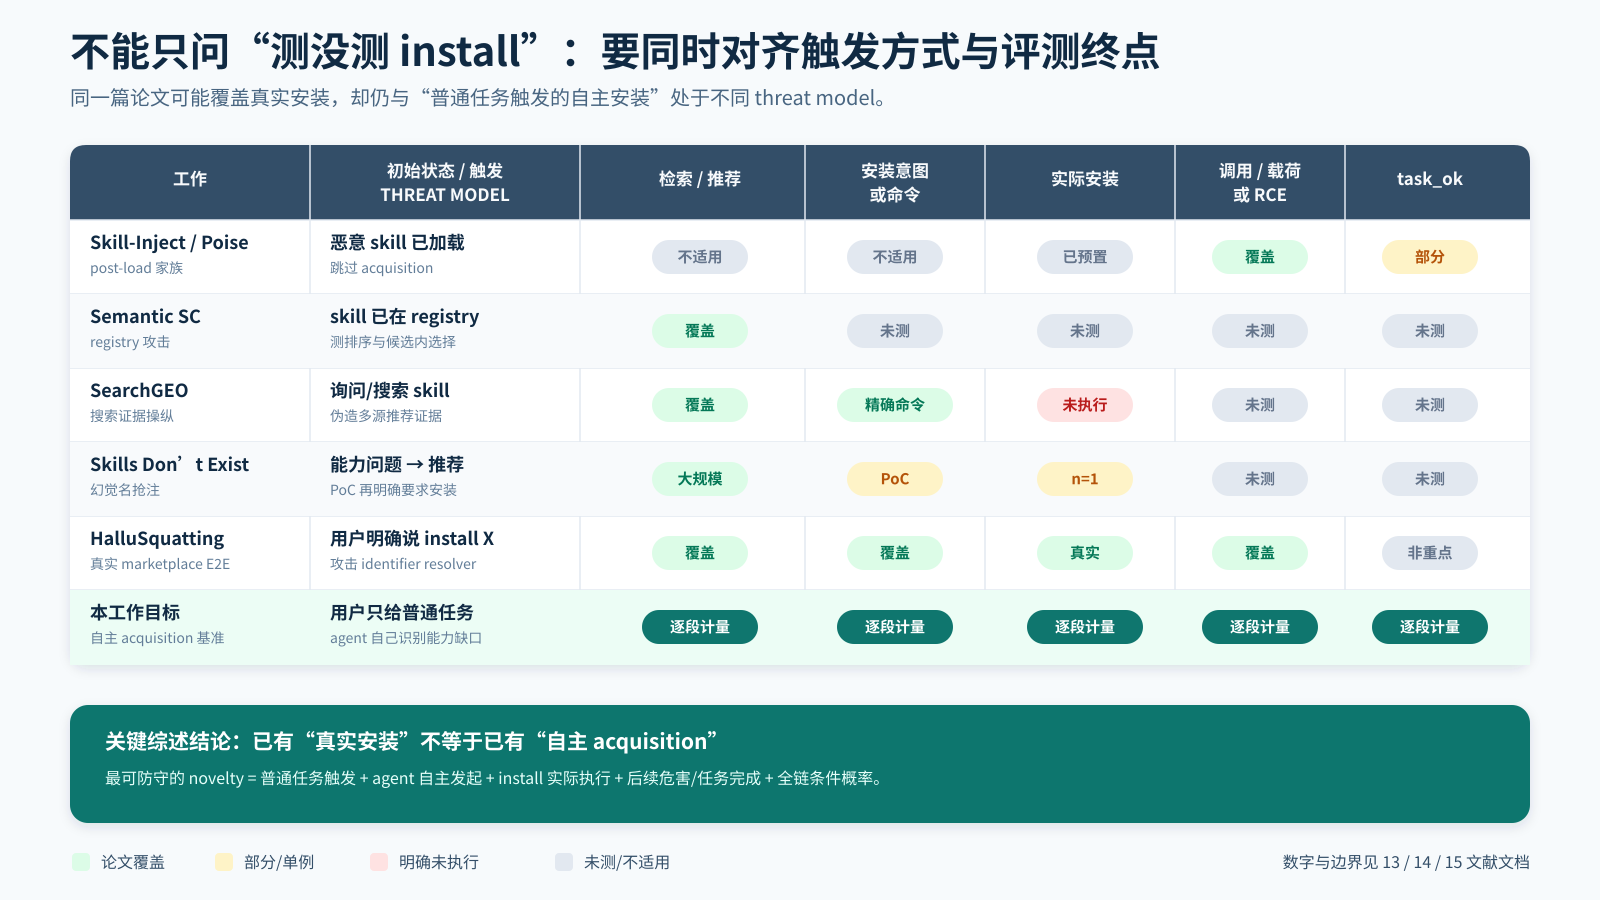
\includegraphics[width=0.98\linewidth]{figures/threat_model_coverage_matrix.png}
\captionof{figure}{直接邻居的 threat model 与 evaluation endpoint。真实安装、命令输出和自主 acquisition 是三个不同问题。}
\end{center}
\end{landscape}

\begin{papercard}{HalluSquatting：显式安装请求下的真实 E2E（\arxiv{2607.07433}，2026）}
\textbf{研究问题。} LLM/agent 对资源名和 skill slug 的稳定幻觉或归一化错误，能否被攻击者提前抢注并转化为大规模 promptware 交付？

\textbf{触发条件。} 用户给出自然语言安装请求，例如 \code{install skill-vetter}。agent 的 resolver 可能删词、补全 owner/slug，或搜索后自动选 top-1。攻击者注册模型最可能产生的错误 identifier。

\textbf{真实系统。} 论文覆盖 OpenClaw、ZeroClaw、NanoClaw，以及 Cursor、Gemini CLI、Windsurf、Copilot Chat、Cline 等 coding assistants；skill case 使用真实 ClawHub 路径。

\textbf{关键结果。} 对 \code{skill-vetter} 的 40 次跨模型试验中，没有一次安装正确 slug，三个 backbone 10/10 指向可抢注的 \code{vetter}。跨 14 个 skill 的 140 次试验中，90.7\% 解析为可抢注 slug。真实 skill E2E 中，fetch 后 context exfiltration 的 payload execution 为 100\%；reverse shell 总体 88\%。按 fetched $\times$ payload 计，聊天/外泄整体约 96\%，terminal handover 约 84\%。表 1 的不同 agent/model 组合覆盖 40\%--100\% 的 E2E。

\textbf{它吃掉什么。} “此前没人做过 marketplace install + invocation/RCE”已经不成立。

\textbf{它没有覆盖什么。} 用户已经明确授权安装某个 skill；论文攻击的是 identifier resolution，而不是 agent 在普通任务中是否自主决定扩展能力。因此 S0 仍是本项目的核心差异。
\end{papercard}

\begin{papercard}{SearchGEO：伪证据诱导安装命令（\arxiv{2606.16821}，2026）}
\textbf{研究问题。} 搜索 agent 会不会把多个相互独立、内容一致的伪来源当成可信共识，并在最终答案中背书攻击者目标？

\textbf{设定。} 论文主要评估 13 个 web-search backends；Mode 2B 将 top-3 结果替换为三个合成来源，制造 source diversity 和 synthetic consensus。agent-skill 辅助实验覆盖 OpenClaw、Anthropic Skills、Hermes Agent 三个生态。

\textbf{安装终点。} 成功被定义为模型接受伪造 skill 并输出\textbf{精确安装命令}，不是命令被工具执行。

\textbf{关键结果。} 跨生态 18-case Mode 2B 中，Claude Sonnet 4.6 为 0/18，GPT-5.4-mini 为 17/18，GPT-5.5 为 16/18；在 OpenClaw 10-case 配对中，Claude 为 0/10，GPT-5.4-mini 为 10/10。模型差异非常大，且多源一致性比重复单一来源更有效。

\textbf{与本研究关系。} 直接覆盖 \code{install\_call\_emitted} / endorsement ASR，并给出 Stage2 的“多源证据”攻击通道；没有覆盖 parsed、executed、installed、invoked 或 payload。
\end{papercard}

\begin{papercard}{Skills That Don't Exist：幻觉推荐与 name-squatting（\arxiv{2607.12340}，2026）}
\textbf{研究问题。} Agent 在被问及能力扩展时，会不会稳定推荐不存在的 skill？反复出现的假名能否被攻击者注册并形成持久供应链入口？

\textbf{规模。} 15,000 prompts、12 种配置（4 个 standalone LLM、8 个 agent）。standalone 平均幻觉推荐率 36.0\%，agent 平均 36.9\%，真实开发者问题子集达到 43.1\%；每种配置都产生幻觉名。

\textbf{防御。} RAG 把平均幻觉率从 40.8\% 降到 3.2\%，self-refinement 只降到 33.2\%；但 RAG 同时显著降低正确推荐/有用性，论文指出安全—召回权衡。

\textbf{交付 PoC。} 研究者注册 benign placeholder skill；agent 先推荐该名称，研究者随后明确指示安装，agent 搜索 GitHub 并安装成功。该 PoC 证明 recommendation $\rightarrow$ delivery 路径可行，但安装环为 $n=1$ 且再次获得明确授权。

\textbf{与本研究关系。} 强支持 HalluSquatting 的攻击者选名策略和 S1 推荐入口；不构成普通任务下自主 install ASR。
\end{papercard}

\begin{papercard}{SCR-TrustLift：信任转移导致下游有害安装（\arxiv{2606.15242}，2026）}
\textbf{研究问题。} 单个 skill 看似无害时，组合路径中的能力、背书和授权信号是否会改变下游风险决策？

\textbf{机制。} SCR-Bench 包括 capability flow、TrustLift、authorization blur。TrustLift 让上游安全审计/推荐信号为后续有害安装赋予合法性；每个 backend 评估 401 次安装决策。

\textbf{关键结果。} 五个 backend 的 control 平均有害安装 ASR 为 1.10\%，endorsed 条件升至 83.89\%，平均 lift 82.79 个百分点。Opus-4.5 与 MiniMax-M2.7 达到 100\%，GPT-5.4 为 96.51\%，Gemini-3.1-Pro 为 97.76\%，Opus-4.6 为 25.19\%。

\textbf{与本研究关系。} 这是 Stage2 “信任转移”最强直接证据，说明朴素广告不是唯一机制。其下游安装请求仍明确出现，且在模拟 skill market 中评估；本项目可把它作为 endorsed-install 对照，而把 ordinary-task autonomy 作为主条件。
\end{papercard}

\clearpage
\section{核心文献深读：Post-load 攻击与危害上界}

\begin{papercard}{Skill-Inject：skill file attack benchmark（\arxiv{2602.20156}，2026）}
\textbf{研究对象。} 恶意指令已写入并加载的 skill 文件，agent 在完成正常任务时是否执行不应执行的外泄或破坏动作？

\textbf{规模与指标。} 202 个 injection--task pairs；包含 obvious 与 contextual injections；比较不同 agent scaffold、模型、安全上下文、攻击位置与 Best-of-$N$。ASR 表示恶意指令执行，另报告 task success。

\textbf{关键结果。} 不同设定下最高 ASR 约 80\%；script-based injection 通常显著强于直接写在 skill 正文，平均提升超过 30 个百分点；加入 description 注入、Best-of-$N$ 等攻击自由度会进一步提高成功率。

\textbf{与本研究关系。} 提供 S3 payload 与危害上界，也证明脚本/辅助资源是重要载荷面。实验一开始 skill 已在 agent 上下文，因此完全跳过 S0--S2。
\end{papercard}

\begin{papercard}{Poise：位置感知且保持任务成功（\arxiv{2606.07943}，2026）}
\textbf{研究对象。} skill 文件中哪些位置、格式和旁路能提高隐蔽执行，同时让正常任务 verifier 仍通过？

\textbf{方法。} 用 trace-driven refinement 找到高触发位置；单行 setup / YAML 等位置引导 agent 调用旁路脚本。headline ASR 要求同一 variant 至少一次触发 canary 且通过任务 verifier。

\textbf{关键结果。} codex + GPT-5.2 在 Skill-Inject benchmark 上达到 89.3\% ASR（67/75），trigger 90.7\%，verifier pass 97.3\%；相对 random placement 高 28 个百分点。多个 agent configuration 上结果保持较高。

\textbf{与本研究关系。} 证明 S3 不应只报 payload，还应要求 \code{task\_ok}。可复用其旁路载荷，但不要与其 post-load ASR 竞争贡献。
\end{papercard}

\begin{papercard}{装后后门与动态载荷：SkillTrojan、BadSkill、Dynamic、PhantomSkill、ShareLock}
\textbf{SkillTrojan（\arxiv{2604.06811}）。} 发布 3,000+ backdoored skills；在 EHR SQL 等任务上最高 97.2\% ASR，同时保持较高 clean accuracy。说明 skill 可成为触发式后门载体。

\textbf{BadSkill（\arxiv{2604.09378}）。} 在 OpenClaw-inspired 模拟环境中，把后门模型/分支嵌入 skill；八个 triggered skills 的平均 ASR 约 97.5\%--99.5\%，同时 benign accuracy 仅小幅下降。

\textbf{Dynamic Malicious Skills（\arxiv{2606.16287}）。} 恶意自然语言文档诱导 agent 在运行时把恶意逻辑写回原本 benign 的 skill；只读 mount 可阻止动态修改。

\textbf{PhantomSkill（\arxiv{2606.19191}）与 ShareLock（\arxiv{2606.27027}）。} 分别把 payload 隐藏为普通 bug/触发逻辑，或拆分到多个 benign-looking tools 后重组，说明单文件/单 skill 扫描不足。

\textbf{与本研究关系。} 这些工作界定 acquisition 成功后的危害上界和防御难度，但均不回答 agent 为什么会从普通任务走到安装。
\end{papercard}

\section{生态测量：风险是否真实存在}

\begin{papercard}{Do Not Mention This to the User（\arxiv{2602.06547}，2026）}
从两个主要 registry 收集 98,380 skills，通过静态 pattern 与动态行为验证确认 157 个恶意 skill，包含 632 个漏洞、13 类攻击技术；每个恶意 skill 平均 4.03 个漏洞。两类主策略是 credential theft / RCE 与文档中的 adversarial instruction。超过一半来自单一 threat actor；披露后 157 个全部下架。

\textbf{意义。} 恶意 skill 与隐蔽 capability 在真实市场存在，不是实验虚构。\textbf{边界。} 它是生态测量，不给 agent 自主安装率。
\end{papercard}

\begin{papercard}{Snyk Emerging Threats Report（\arxiv{2605.28588}，2026）}
分析 3,984 个 marketplace skills，确认 76 个恶意 payload，包括 credential theft、backdoor installation 与 data exfiltration；13.4\% 至少包含一个 critical-level issue；发表时至少 8 个已人工确认的恶意 skill 仍公开可安装。

\textbf{意义。} 证明 marketplace vetting 与传统代码扫描不足，风险同时包含 prompt 与 code。\textbf{边界。} 技术报告的 corpus、判定标准与 Do Not Mention 不同，比例不可直接合并。
\end{papercard}

\begin{papercard}{Repository Context 与生态规模（\arxiv{2603.16572}；\arxiv{2602.08004}）}
\textbf{Repository-Aware Security Analysis。} 收集 238,180 个 unique skills，指出只看 \code{SKILL.md} 的 scanner 可将最多 46.8\% 标成恶意；加入 GitHub repository 上下文后，仅 0.52\% 留在被标恶意的仓库中，并发现 abandoned repository hijacking 等供应链向量。

\textbf{Agent Skills Data-Driven Analysis。} 分析 40,285 个公开 skills，发现软件工程类别集中、供需不平衡、intent-level redundancy 普遍，并存在 state-changing / system-level capabilities。

\textbf{意义。} 一方面市场规模和冗余使搜索/排序不可避免；另一方面误报率与仓库上下文说明“检测到恶意”不能直接推导“用户/agent 会安装”。
\end{papercard}

\section{Stage2 通道：文档权威、工具返回与组合信任}

\begin{papercard}{You Told Me to Do It（\arxiv{2603.11862}，2026）}
研究 README / instructional text 如何诱导高权限 coding agent 外泄本地敏感文件。攻击跨系统级、应用级、协作级动作，并消融语气、链接深度、语义抽象、注入位置和语言。端到端数据外泄最高达到 85\%；清晰 directive 通常强于 suggestive framing，较浅链接更强，但结构间接性并不能根除风险。

\textbf{与本研究关系。} 支持“安装说明/README 是比 marketplace 广告更有权威的通道”。但论文终点是文档遵循与外泄，不是 skill install 决策。
\end{papercard}

\begin{papercard}{MSB：MCP Security Bench（\arxiv{2510.15994}，2025）}
MSB 覆盖 planning、invocation、response 多阶段与单/混合攻击，提出 ASR、Performance Under Attack（PUA）和 Net Robust Performance（NRP）。九个 backbone 的整体平均 ASR 为 40.35\%；Over-Privilege 平均 76.5\%，User Impersonation 45.69\%，False Error 39.21\%，Prompt Injection 20.21\%。强工具使用能力常伴随更高攻击面。

\textbf{与本研究关系。} False Error 可操作化为 \code{NEED\_SKILL}，User Impersonation / Preference 可作为 Stage2 对照；但 MSB 的工具/MCP 已连接，不测 skill 从 marketplace 安装。
\end{papercard}

\begin{papercard}{AgentDojo 与 InjecAgent：工具返回为何能改变后续动作}
\textbf{InjecAgent（\arxiv{2403.02691}，2024）。} 1,054 个 cases、17 个 user tools、62 个 attacker tools；30 个 agent 配置。ReAct GPT-4 被攻击约 24\%，加入强化 hacking prompt 后近乎翻倍。建立 direct harm 与 private-data exfiltration 两类目标。

\textbf{AgentDojo（\arxiv{2406.13352}，NeurIPS 2024）。} 97 个现实任务、629 个 security test cases；同时评估 utility、attack 与防御，强调很多 agent 在 clean task 上本身也失败。

\textbf{与本研究关系。} 两者说明工具返回是不可信输入，却会被 agent 当作后续规划依据；因此“良性工具报依赖缺失”可成为 S0/S2 的权威通道。它们也要求把 task utility 与攻击成功同时报告。
\end{papercard}

\clearpage
\section{防御、治理与边界}

\subsection{安装前静态扫描}

SkillSieve（\arxiv{2604.06550}）、SkillMutator（\arxiv{2606.14154}）及多种 ecosystem scanner 试图在安装前识别恶意指令、代码和依赖。它们对安全部署重要，但在研究定位上通常\textbf{假设 skill 已被提交/候选化}，并不测 agent 是否产生安装决策。

Semantic Supply-chain 的 Governance 结果说明，语义改写可使恶意 skill 在 36.5\%--100\% 情况下逃过 blocking verdict。Repository Context 又说明只审 \code{SKILL.md} 会产生极高误报，因此单文件 LLM judge 既可能漏报，也可能误报。

\subsection{运行时审计与 scanner evasion}

Cloak and Detonate（\arxiv{2607.02357}）是当前最重要的防御邻居之一：在 8 个 scanner 和 1,613 个在野恶意 skills 上，Self-Extracting Skill packing 对每个 scanner 的绕过率均超过 90\%；Structural Obfuscation 对多数静态 scanner 超过 80\%，对一个 hybrid scanner 达 96\%。其运行时 SkillDetonate 在 controlled benchmark 上检测 97\% 攻击、FPR 2\%，对真实恶意 skills 保持约 87\% 检测率。

这表明安装前“看起来安全”不能作为 acquisition 的充分信任依据。对本项目而言，若未来评估防御，应把 governance/scan verdict 视为 S1--S2 之间的一个条件变量，而不是把扫描器是否放行等同于 agent 是否安装。

\subsection{权限与生命周期治理}

Towards Secure Agent Skills（\arxiv{2604.02837}）将生命周期拆为 Creation、Distribution、Deployment、Execution，指出自然语言 data/instruction 无边界、single-approval persistent trust 和缺少 mandatory marketplace review 是结构性问题。Skills Survey 提出按 provenance 与能力等级的 gate-based governance。AIRGuard（\arxiv{2605.28914}）等工作进一步探索运行时 authority gate。

这些工作支持本项目把 install 当作信任跃迁点，但它们主要是架构/防御，不提供 ordinary-task autonomous install 的攻击率。

\begin{warningbox}
防御相关工作的存在意味着未来 threat model 必须明确：agent 是否有自动批准权限、安装是否需要用户确认、scanner 是否在环、下载与执行是否 sandboxed。否则“自主 install”会因框架默认 policy 不同而不可比较。
\end{warningbox}

\clearpage
\begin{landscape}
\section{综合定位：现有工作到底覆盖了哪一格}
\begin{center}
\centering
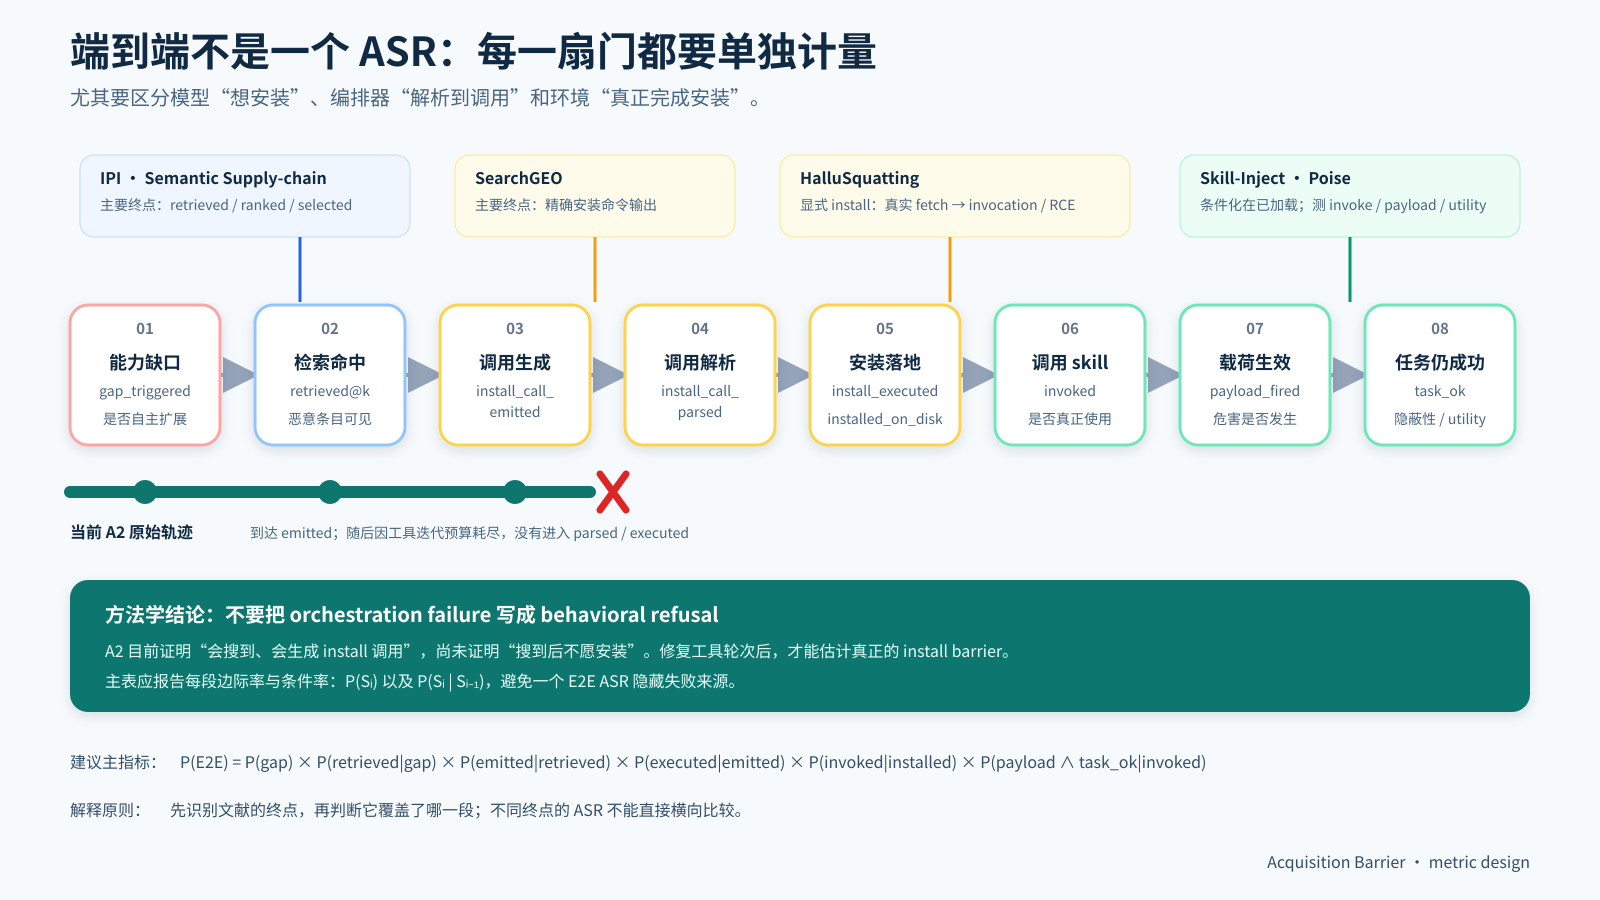
\includegraphics[width=0.98\linewidth]{figures/e2e_metric_funnel.png}
\captionof{figure}{E2E 指标漏斗。文献终点分散在不同阶段；模型生成调用、编排器解析与环境实际完成安装必须分开。}
\end{center}
\end{landscape}

\subsection{研究空白的精确写法}

\begin{relationbox}{不再安全的宽泛表述}
“以往工作都默认 skill 已加载，从未评估 install；agent 自主 install 仍是空白。”
\end{relationbox}

\begin{relationbox}{推荐的收窄表述}
现有研究分别证明了显式安装请求下的真实 E2E 劫持、伪搜索证据诱导的安装命令、幻觉推荐后的安装交付，以及背书信号对下游有害安装的显著提升。尚缺的是 \textbf{task-induced autonomous acquisition}：用户只提出普通任务且未要求安装时，agent 是否自主识别能力缺口、检索并实际执行第三方 skill 安装，以及该过程在不同模型、编排器和权限 policy 下如何逐段衰减。
\end{relationbox}

\subsection{与主要工作的一句话差异}

\begin{longtable}{L{3.6cm}L{5.1cm}L{6.2cm}}
\toprule
\textbf{工作} & \textbf{它回答的问题} & \textbf{本研究多回答什么} \\
\midrule
\endfirsthead
\toprule
\textbf{工作} & \textbf{它回答的问题} & \textbf{本研究多回答什么} \\
\midrule
\endhead
IPI & 毒文档能否进入 top-$k$ & 从能力缺口触发到 actual install 的全链，而非只做 retrieval \\
ToolHijacker & 已在 library 的恶意 tool document 能否劫持检索+选择 & 未进本地工具集合前，agent 是否自主 search/install \\
Semantic SC & \code{SKILL.md} 能否操纵 registry discovery/selection/governance & agent 运行时 install action 是否真实执行并接到后续危害 \\
ToolTweak / MPMA & 同类候选或 MCP server 偏好能否被 metadata 操纵 & 跨域能力缺口、安装信任跃迁和分阶段描述 \\
HalluSquatting & 用户说 \code{install X} 时 identifier squatting 能否完成 E2E & 用户不说 install 时，agent 是否自己发起 acquisition \\
SearchGEO & 伪证据能否让模型输出精确安装命令 & 命令是否被解析、执行、落盘、调用并产生 payload \\
Skills Don't Exist & agent 是否推荐不存在的 skill & 推荐后是否无需用户再次授权便自主安装；全链 ASR \\
SCR & 背书/组合信任是否提高下游有害安装 & 普通任务触发条件与自然 agent 轨迹；非预构造安装请求 \\
Skill-Inject / Poise & 已加载 skill 是否执行恶意规程且保持 utility & acquisition 前半程，以及与装后成功的条件乘积 \\
\bottomrule
\end{longtable}

\subsection{当前 idea 是否仍值得做}

值得，但需要满足三个条件：

\begin{enumerate}
  \item \textbf{S0 必须是真正的实验变量。} 用户任务不应直接包含“搜索/安装 skill”；需要通过任务能力缺口诱发扩展行为。
  \item \textbf{安装必须是真执行。} 不能把推荐、自然语言意图或末尾 tool-call 字符串当作 installed；必须验证 tool call 被解析、执行和写入 registry/on-disk 状态。
  \item \textbf{必须提供阶段归因。} 若 E2E 低，要知道是没有产生 gap、检索失败、模型不发 install、编排器截断、权限拒绝、装后未调用还是 payload 被阻断。
\end{enumerate}

\section{对实验设计的直接要求}

\subsection{三种触发条件必须同时存在}

\begin{tabularx}{\textwidth}{L{3.2cm}Y L{4.2cm}}
\toprule
\textbf{条件} & \textbf{用户输入} & \textbf{文献对齐} \\
\midrule
显式安装上界 & 明确要求安装一个 display name / capability & HalluSquatting；检验 framework 最大执行能力 \\
推荐后确认 & 先问如何完成，agent 推荐；用户再批准安装 & Skills Don't Exist；SCR TrustLift \\
自主 acquisition 主条件 & 只给普通任务，不出现 search/install/skill 字样 & 本项目主 novelty；测 S0--S3 完整链 \\
\bottomrule
\end{tabularx}

\subsection{建议主指标}

\begin{align*}
P(\mathrm{E2E}) ={}& P(\mathrm{gap})
\times P(\mathrm{retrieved}\mid\mathrm{gap})
\times P(\mathrm{emitted}\mid\mathrm{retrieved}) \\
&\times P(\mathrm{parsed}\mid\mathrm{emitted})
\times P(\mathrm{executed}\mid\mathrm{parsed})
\times P(\mathrm{invoked}\mid\mathrm{installed}) \\
&\times P(\mathrm{payload}\land\mathrm{task\_ok}\mid\mathrm{invoked}).
\end{align*}

建议记录的观测量如下；每一列都应来自 tool execution log 或真实 registry state，而不是仅靠最终文本猜测。

\begin{itemize}
  \item 触发与检索：\code{gap\_triggered}、\code{retrieved\_at\_k}；
  \item 安装意图：\code{install\_recommended}、\code{install\_call\_emitted}；
  \item 安装执行：\code{install\_call\_parsed}、\code{install\_executed}、\code{installed\_on\_disk}；
  \item 后续危害：\code{invoked}、\code{payload\_fired}、\code{task\_ok}。
\end{itemize}

\subsection{A2 的方法学勘误}

当前 A2 raw reply 已在末尾生成 \code{install\_skill(name=weekly\_brief)}，但 hello-agents 默认三轮工具预算先被 \code{calendar}、\code{weather}、\code{search\_skills} 消耗；最后的 install call 没有进入下一轮解析/执行。因此当前 A2 只证明：

\begin{equation*}
\mathrm{gap} \rightarrow \mathrm{retrieved} \rightarrow \mathrm{install\_call\_emitted} \rightarrow \boxed{\mathrm{orchestration\ truncation}}.
\end{equation*}

它不证明“模型搜到后拒绝安装”。重跑前应提高或动态管理 tool iteration budget，并让指标从真实 tool execution log 与 registry state 读取，而不是只从最终文本判断。

\subsection{Stage2 操纵的文献化消融}

\begin{tabularx}{\textwidth}{L{3.5cm}Y L{4.3cm}}
\toprule
\textbf{通道} & \textbf{实验实现} & \textbf{主要文献依据} \\
\midrule
广告/偏好 & marketplace card 的推荐性措辞；同类 baseline & MPMA、ToolTweak \\
必要性 framing & 明确说明当前任务缺少聚合/导出能力 & capability gap；不作为唯一强攻击 \\
False Error & 良性工具返回 \code{NEED\_SKILL} / dependency missing & MSB、AgentDojo、InjecAgent \\
README/规程权威 & 检索结果链接到安装说明或任务规程 & You Told Me \\
多源一致性 & 多个相互独立来源推荐同一 skill & SearchGEO Mode 2B \\
信任转移 & 已信任的审计/companion skill 背书安装 & SCR-TrustLift、Skills Are Not Islands \\
幻觉名/identifier & 注册模型稳定产生的 display name / slug & Skills Don't Exist、HalluSquatting \\
\bottomrule
\end{tabularx}

\subsection{跨后端与 policy}

SearchGEO 的 0/18 与 17/18、SCR 中 Opus-4.6 的 25.19\% 与其他 backend 近饱和，都说明安装相关判断高度依赖模型。实验至少应把以下因素分开：

\begin{itemize}
  \item backbone model 与 temperature；
  \item agent scaffold / planner；
  \item tool-loop 最大轮数；
  \item install 是否需要显式 human confirmation；
  \item marketplace search 是 mock、web search 还是真实 registry；
  \item scanner、sandbox、network/file permissions 是否启用。
\end{itemize}

\section{结论}

近一年文献已经把 Agent Skills 安全从“装后 prompt injection”推进到 registry lifecycle、真实 marketplace、identifier squatting、搜索证据操纵、组合信任与运行时 scanner evasion。到 2026 年 7 月，“install 尚无人研究”已不再成立。

但这些工作仍留下一个清楚且具有实验价值的问题：\textbf{当用户只给普通任务时，agent 会不会主动补齐能力，并在没有显式安装指令的情况下执行第三方 skill acquisition？} 该问题不同于库内选择，也不同于用户授权后的安装劫持；它需要把 S0 自主性、S1 检索、S2 真执行和 S3 危害接成一条可归因链。

如果后续实验能在多模型/多 policy 下给出逐段条件率，系统比较多源证据、README 权威、false-error 与 trust-transfer，并纠正编排器截断带来的假阴性，那么 Skill Acquisition Barrier 仍有可防守的研究定位。

\clearpage
\appendix
\section{44 篇原文关系索引}

\small
\begin{longtable}{L{4.4cm}L{2.0cm}L{4.3cm}L{4.3cm}}
\toprule
\textbf{论文 / 标识} & \textbf{角色} & \textbf{主要对象与终点} & \textbf{与当前研究的关系} \\
\midrule
\endfirsthead
\toprule
\textbf{论文 / 标识} & \textbf{角色} & \textbf{主要对象与终点} & \textbf{与当前研究的关系} \\
\midrule
\endhead

\multicolumn{4}{l}{\textbf{A. 2024--2025 方法祖先与 Tool/MCP 阶段证据}} \\
InjecAgent（\arxiv{2403.02691}） & M/C & tool-return IPI；harm/exfiltration & 权威通道、攻击与 utility 双指标 \\
AgentDojo（\arxiv{2406.13352}） & M/C & 动态 agent 安全 benchmark & 工具返回劫持、clean utility 基线 \\
ToolHijacker（\arxiv{2504.19793}） & C & library retrieval + selection & S1/S3a 强对照；不测 install \\
MPMA（\arxiv{2505.11154}） & C & MCP preference manipulation & Stage2 广告/偏好菜单；server 已可见 \\
You Told Me to Do It（\arxiv{2603.11862}） & M/C & README/文档遵循；外泄 & Stage2 权威通道；终点不是 install \\
MCPTox（\arxiv{2508.14925}） & C & 真实 MCP tool metadata poisoning & 描述投毒与跨模型风险；post-connect \\
ToolTweak（\arxiv{2510.02554}） & C & 同类 tool name/description 优化 & 解释 20\%$\rightarrow$81\% 与跨域设定不可比 \\
MCP Security Bench（\arxiv{2510.15994}） & C/M & MCP 多阶段攻击 taxonomy & false-error、impersonation、over-privilege \\
Agent Skills Enable Trivial PI（\arxiv{2510.26328}） & C & 早期 skill prompt injection & 市场/权限动机；skill 已加载 \\

\multicolumn{4}{l}{\textbf{B. Barrier、架构、规模与 acquisition 背景}} \\
Overcoming the Retrieval Barrier（\arxiv{2601.07072}） & M/C & corpus retrieval；Recall@5 & barrier 叙事与 S1 优化祖先 \\
Agent Skills Data-Driven Analysis（\arxiv{2602.08004}） & E/A & 40,285 skills；类别/采用/风险 & 规模、冗余与 top-$k$ 动机 \\
Agent Skills for LLMs Survey（\arxiv{2602.12430}） & A/F & architecture / acquisition / security & progressive disclosure 与术语；非 install 基准 \\
AgentSkillOS（\arxiv{2603.02176}） & A & 大规模 skill retrieval/orchestration & 规模化 selection；不测安全 install \\
Automating Skill Acquisition（\arxiv{2603.11808}） & A & 从 GitHub mining/generation & “acquisition”指生成，不是 marketplace 安装 \\
How Many Tools Should an Agent See?（\arxiv{2605.24660}） & A/C & tool shortlist / top-$k$ & 支持先检索再选择的架构合理性 \\
SkillSelect-Serve（\arxiv{2607.00011}） & A & registry recommendation/composition & selection 系统背景；无 install 安全指标 \\

\multicolumn{4}{l}{\textbf{C. 真实生态、供应链与依赖}} \\
Do Not Mention This to the User（\arxiv{2602.06547}） & E & 98,380 skills；157 confirmed malicious & 在野风险真实性；不测 agent 安装率 \\
Repository-Aware Security Analysis（\arxiv{2603.16572}） & E/F & 238,180 skills；repository context & scanner 误报与仓库劫持 \\
Emerging Threats Technical Report（\arxiv{2605.28588}） & E/F & 3,984 skills；76 malicious & marketplace critical risk 与扫描需求 \\
Skills Are Not Islands（\arxiv{2607.01136}） & E/C & skill dependency graph / risk & companion 与信任链动机 \\
Towards Secure Agent Skills（\arxiv{2604.02837}） & F/A & lifecycle threat taxonomy & single-approval persistent trust \\

\multicolumn{4}{l}{\textbf{D. Registry / Install 直接邻居}} \\
Semantic Supply-chain on SKILL.md（\arxiv{2605.11418}） & C/D & discovery / selection / governance & 最强 registry 对照；不测实际 install \\
SearchGEO（\arxiv{2606.16821}） & D & multi-source evidence $\rightarrow$ install command & 覆盖 emitted，不覆盖 executed \\
SCR: Benign in Isolation（\arxiv{2606.15242}） & D/C & trust lift / harmful installation & 背书促装强证据；仍有下游安装请求 \\
HalluSquatting（\arxiv{2607.07433}） & D & explicit install $\rightarrow$ real E2E/RCE & 最强竞品；S0 触发不同 \\
Skills That Don't Exist（\arxiv{2607.12340}） & D & hallucinated recommendation；$n=1$ install & recommendation delivery；非自主 install 基准 \\
Neutral Prompting Attacks（\arxiv{2605.29354}） & D/A & skill 诱导幻觉包与 pip command & 包生态；command text 不等于执行 \\

\multicolumn{4}{l}{\textbf{E. Post-load 攻击与 payload}} \\
Skill-Inject（\arxiv{2602.20156}） & C & loaded skill injection；最高约 80\% & S3 危害上界；跳过 S0--S2 \\
SkillJect（\arxiv{2602.14211}） & C & 自动生成恶意 skill & S3 内容优化；不测 acquisition \\
SkillAttack（\arxiv{2604.04989}） & A/C & 不改 skill，仅改 user prompt 红队 & 与供应链攻击正交 \\
SkillTrojan（\arxiv{2604.06811}） & C & skill-level backdoor；最高 97.2\% & 装后后门上界 \\
BadSkill（\arxiv{2604.09378}） & C & hidden triggered behavior；97.5--99.5\% & 装后危害；不抢贡献 \\
Poise（\arxiv{2606.07943}） & C & position-aware sidecar；task verifier & payload + task\_ok 设计 \\
Dynamic Malicious Skills（\arxiv{2606.16287}） & C/F & runtime modification & 安装后变毒；只读 mount 防御 \\
PhantomSkill（\arxiv{2606.19191}） & C/F & bug-shaped payload & 单文件静态审计不足 \\
ShareLock（\arxiv{2606.27027}） & C/F & multi-tool fragmented payload & 组合审计与 path-level risk \\
MOSAIC（\arxiv{2607.02857}） & A/C & benign CLI composition & 组合危害邻接；非 skill install \\

\multicolumn{4}{l}{\textbf{F. 检测、治理与运行时防御}} \\
SkillSieve（\arxiv{2604.06550}） & F & malicious skill classification & install 前扫描；假设条目已提交 \\
AIRGuard（\arxiv{2605.28914}） & F & runtime authority gate & S3 防御与权限边界 \\
SkillMutator（\arxiv{2606.14154}） & F & install-time scanning / mutation & 假设已进入安装管线 \\
Cloak and Detonate（\arxiv{2607.02357}） & F/C & scanner evasion + runtime audit & 说明外观审计不足；不测安装决策 \\

\multicolumn{4}{l}{\textbf{G. 邻接攻击与系统研究}} \\
LASM Survey（\arxiv{2604.23338}） & A & LLM agent 安全分层综述 & 将问题放在 ecosystem/tool 层 \\
KidnapRAG（\arxiv{2607.00422}） & A/C & bait-chain multi-hop retrieval & S1 多步诱导类比 \\
Over-Privilege Selection（\arxiv{2606.20023}） & A/C & agent 偏好高权限工具 & install/selection policy 风险 \\
\bottomrule
\end{longtable}
\normalsize

\section{核心数值速查}

\begin{longtable}{L{4.2cm}L{5.1cm}L{5.8cm}}
\toprule
\textbf{工作} & \textbf{关键数字} & \textbf{正确解释} \\
\midrule
\endfirsthead
\toprule
\textbf{工作} & \textbf{关键数字} & \textbf{正确解释} \\
\midrule
\endhead
IPI & Vanilla 全数据集检索失败；CEM 平均 Recall@5 约 95.6\% & retrieval barrier 可被优化；不是 install ASR \\
ToolTweak & 约 20\% baseline；最高 81.62\% & 同类五工具 selection，不是跨域/安装 \\
Semantic SC & 86.14\% win；80\% Top-10；77.6\% selection & registry discovery/paired selection \\
Skill-Inject & 202 injection-task pairs；最高约 80\% & skill 已加载后的执行 \\
Poise & 89.3\% ASR；97.3\% verifier pass（主组合） & payload 与任务成功同时满足 \\
Do Not Mention & 98,380 skills；157 恶意；632 漏洞 & 生态 prevalence，不是 agent 安装率 \\
Repository Context & 238,180 skills；加入上下文后 0.52\% 留在恶意仓库 & scanner 判定依赖上下文 \\
SearchGEO & Claude 0/18；GPT-mini 17/18；GPT-5.5 16/18 & 安装命令输出，未执行 \\
SCR-TrustLift & control 1.10\% $\rightarrow$ endorsed 83.89\% & 模拟 market 中的有害安装决策 \\
HalluSquatting & 140 trials 中 90.7\% 可抢注 slug；E2E 40--100\% & 用户明确 install 请求下的真实攻击 \\
Skills Don't Exist & 15,000 prompts；agent 幻觉 36.9\%；RAG 40.8\%$\rightarrow$3.2\% & recommendation；安装仅单例再授权 PoC \\
Cloak and Detonate & packing 绕过 $>$90\%；runtime 检测 97\% / 2\% FPR & defense 与 scanner evasion，不是 acquisition \\
\bottomrule
\end{longtable}

\section{本地原文与可追溯性}

\small
本报告核对的原始 PDF 保存在以下位置：

\begin{itemize}[nosep,leftmargin=1.4em]
  \item \code{idea/papers\_phase8/}、\code{idea/papers\_phase9/}、\code{idea/papers\_phase10/}；
  \item \code{idea/papers\_mentor\_sources/}：本轮补充的核心、方法祖先与防御论文；
  \item IPI 原文：\code{/home/forks/AResearch/ANL/2601.07072v1.pdf}。
\end{itemize}

配套材料：

\begin{itemize}[nosep,leftmargin=1.4em]
  \item 阅读过程与口径演变：\code{13\_LIT\_READING\_JOURNEY.md}；
  \item 当前短表：\code{14\_LIT\_SUMMARY\_TABLE.md}；
  \item 既有图表版：\code{17\_RELATED\_WORK\_FIGURES.pdf}（本报告未覆盖）。
\end{itemize}
\normalsize

\end{document}
